\documentclass[11pt]{article}
\usepackage{hyperref}
\usepackage[english]{babel}
\usepackage{blindtext}
\usepackage{url}
\usepackage{graphicx}
\usepackage{multicol}
\usepackage[center]{titlesec}
\usepackage{geometry}
\usepackage[T1]{fontenc}
\usepackage[utf8]{inputenc}
\usepackage{lettrine} % The lettrine is the first enlarged letter at the beginning of the text

%\usepackage{mathtools}

\usepackage[sort, numbers]{natbib}


%
%\setlength{\columnseprule}{0.4pt}
%\setlength{\footskip}{20pt}
\usepackage{fancyhdr}
\fancyhf{}
\fancyhead[C]{Valéry Madsen Beau de Rochars $\bullet$ Joe Brew }
\fancyfoot[C]{  $\bullet$ CHIKV \bullet$  }
\renewcommand\headrulewidth{1pt}
\renewcommand\footrulewidth{1pt}
\pagestyle{fancy}

%

\setlength{\columnsep}{1.5cm}
%\setlength{\columnseprule}{0.4pt}

%\MakeOuterQuote{"}



\graphicspath{ {/home/joebrew/Documents/haiti/chik/report} }

%the next two lines adjust the third, centered section of the exec sum
\def\changemargin#1#2{\list{}{\rightmargin#2\leftmargin#1}\item[]}
\let\endchangemargin=\endlist 

\usepackage{Sweave}
\begin{document}
\Sconcordance{concordance:chik_analyse_pour_madsen.tex:chik_analyse_pour_madsen.Rnw:%
1 44 1 1 0 2 1 1 19 8 1 1 7 1 2 61 1 1 22 1 3 24 1 1 19 1 2 21 1 1 25 1 %
3 22 1 1 21 1 5 21 1 1 22 1 4 45 1 1 51 1 2 17 1}




\title{\textbf{Première analyse des données du chikungunya}}
\author{Joe Brew}


\maketitle

\begin{center}
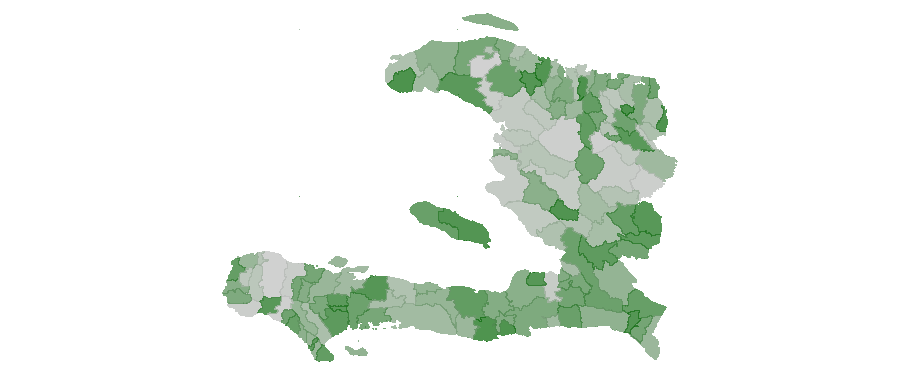
\includegraphics{chik_analyse_pour_madsen-002}
\end{center}

\tableofcontents

%\vspace{20mm}

\begin{center}

\includegraphics[width=2cm]{uf}
\end{center}


\newgeometry{margin=2.5cm}
%\fancyhfoffset[E,O]{0pt}

%------------------------------------------
\section*{Résumé des données de chikungunya}
\addcontentsline{toc}{section}{Résumé des données de chikungunya}
%------------------------------------------
\hrulefill

\begin{multicols}{2} 
\setkeys{Gin}{width=0.45\textwidth}

%------------------------------------------
\subsection*{Panorama}
\addcontentsline{toc}{subsection}{Panorama}
%------------------------------------------

\lettrine[nindent=0em,lines=3]{C}{eci} est une analyse préliminaire des données du chikungunya (CHIKV).  Il s'agit d'un résumé court des documents envoyés a Joe par Madsen le 6 de novembre, 2014, répondant spécifiquement aux sujets délignés par Madsen le même jour.\footnote{1. First merge them by Child code 2. Round a first analysis on the following variables Sex, age, grade, temperature, Age X CHIKV RST, Sex X Age X CHIKV RST}

\vfill
\columnbreak
%------------------------------------------
\subsection*{Introduction}
%------------------------------------------


This is a preliminary analysis of the chikungunya data.  It consists of a brief summary of the documents which Madsen sent to Joe on November 6, 2014, responding specifically to the questions Madsen laid out in his email of the same date.  

\end{multicols}
\setkeys{Gin}{width=1\textwidth}
\begin{multicols}{2} 
\setkeys{Gin}{width=0.45\textwidth}


%------------------------------------------
\subsection*{Sexe}
\addcontentsline{toc}{subsection}{Sexe}
%------------------------------------------
Une majorité petite des observations appartiennent à des filles (54\%).

\vfill
\columnbreak

%------------------------------------------
\subsection*{Sex}
%------------------------------------------
A small majority of observations are from girls (54\%).

\end{multicols}
\setkeys{Gin}{width=1\textwidth}
\begin{center}
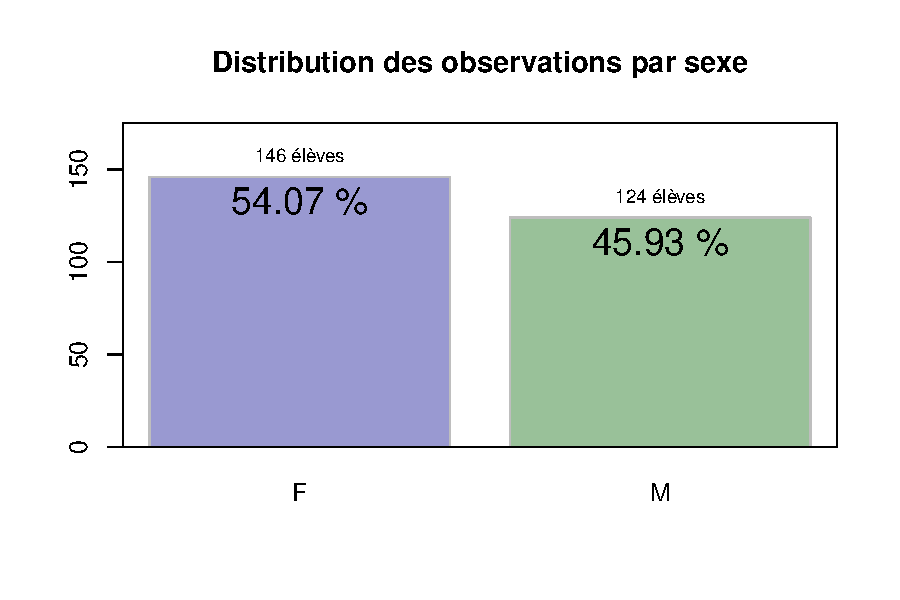
\includegraphics{chik_analyse_pour_madsen-003}
\end{center}

\newpage
\begin{multicols}{2} 
\setkeys{Gin}{width=0.45\textwidth}


%------------------------------------------
\subsection*{Age}
\addcontentsline{toc}{subsection}{Age}
%------------------------------------------
Les élèves ont entre 3 et 22 ans (écart interquartile de 7 a 13 ans)

\vfill
\columnbreak

%------------------------------------------
\subsection*{Age}
%------------------------------------------
Students range from between 3 and 22 years of age (interquartile range of 7 to 13).


\end{multicols}
\setkeys{Gin}{width=1\textwidth}
\begin{center}
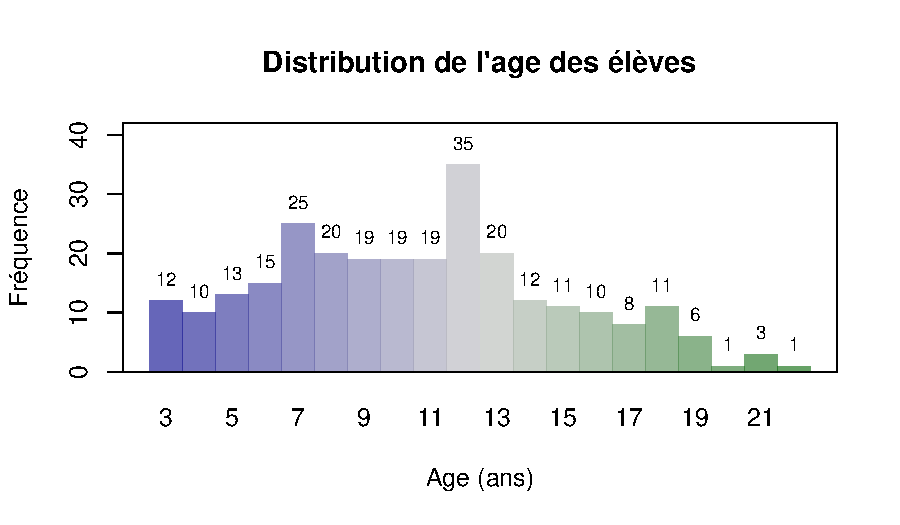
\includegraphics{chik_analyse_pour_madsen-004}
\end{center}
\begin{multicols}{2} 
\setkeys{Gin}{width=0.45\textwidth}


%------------------------------------------
\subsection*{Grade}
\addcontentsline{toc}{subsection}{Grade}
%------------------------------------------
Il y a une distribution presque égale entre les élèves de primaire et secondaire; moins de 20\% viennent de kinder.  

\vfill
\columnbreak

%------------------------------------------
\subsection*{Grade}
%------------------------------------------
There is a nearly even distribution of students in primary and secondary school; fewer than 20\% come from kindergarten.

\end{multicols}
\setkeys{Gin}{width=1\textwidth}
\begin{center}
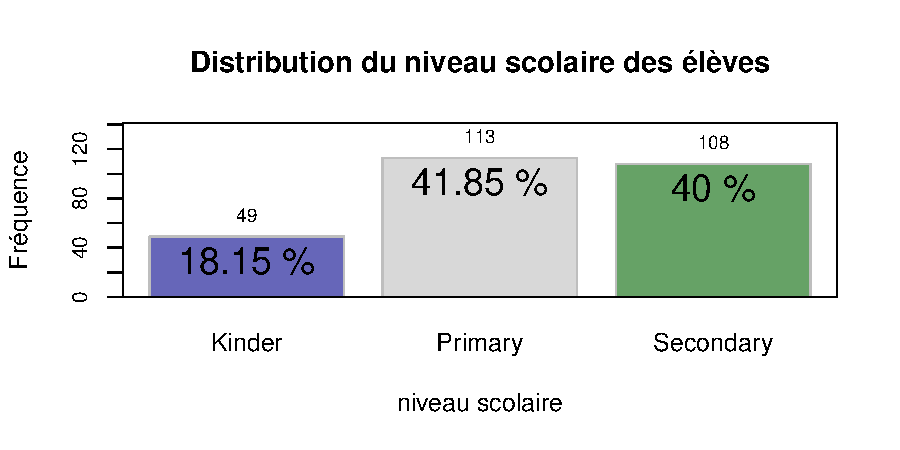
\includegraphics{chik_analyse_pour_madsen-005}
\end{center}
\begin{multicols}{2} 
\setkeys{Gin}{width=0.45\textwidth}



%------------------------------------------
\subsection*{Température}
\addcontentsline{toc}{subsection}{Température}
%------------------------------------------
Une majorité des élèves (170 de 270) avaient une température élévée (plus de 38 C).

\vfill
\columnbreak

%------------------------------------------
\subsection*{Temperature}
%------------------------------------------
A majority of students (170 of 270) had an elevated temperature (greater than 38 C).

\end{multicols}
\setkeys{Gin}{width=1\textwidth}
\begin{center}
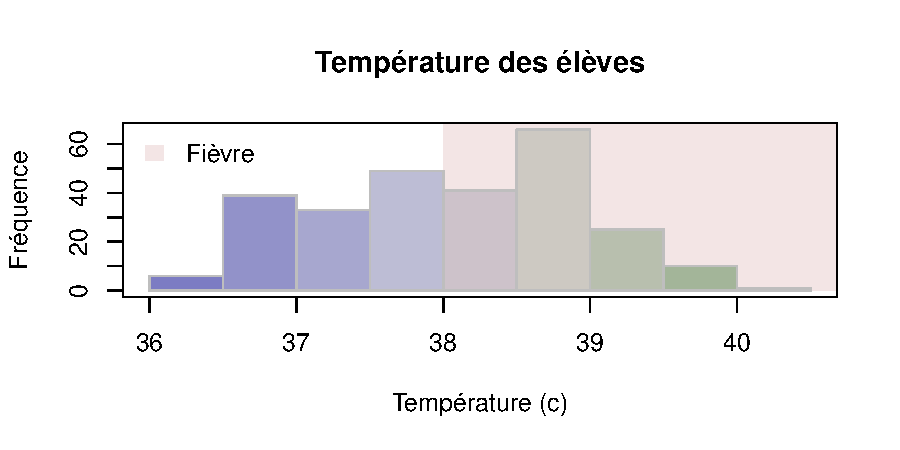
\includegraphics{chik_analyse_pour_madsen-006}
\end{center}
\begin{multicols}{2} 
\setkeys{Gin}{width=0.45\textwidth}



%------------------------------------------
\subsection*{Associations entre les deux feuilles de calcul}
\addcontentsline{toc}{subsection}{Associations entre les deux feuilles de calcul}
%------------------------------------------
\textbf{Important:} Des 270 élèves, seulement 68 sont associés avec un résultat de test (les autres 55 résultats ont des "child codes" qui n'éxistent pas dans le roster des élèves).  Par conséquent, les  mises en tableaux qui suivent ne se prêtent pas a l'interprétation sans de la précaution.
\vfill
\columnbreak

% %------------------------------------------
% \subsection*{Matches between the two spreadsheets}
% %------------------------------------------
% \textbf{Important:} Of the 270 students, only 67 are associated with a test result (the other 55 test results have "child codes" which do not exist in the student roster).  Therefore, the following cross-tabulations should be interpreted with caution.

\end{multicols}
\setkeys{Gin}{width=1\textwidth}
\begin{center}
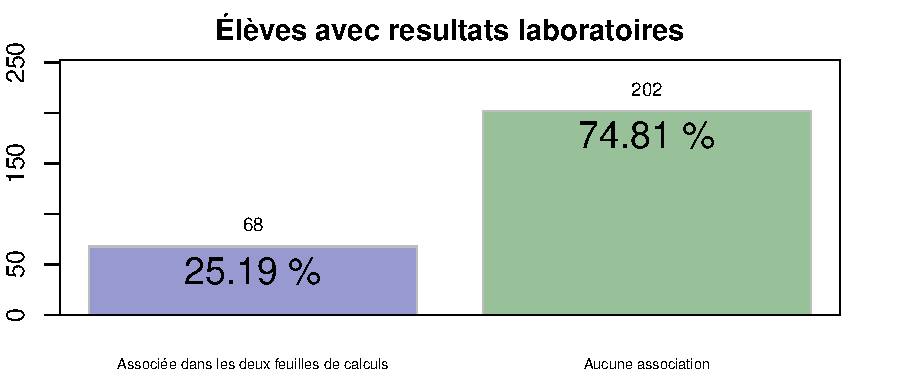
\includegraphics{chik_analyse_pour_madsen-007}
\end{center}
\begin{multicols}{2} 
\setkeys{Gin}{width=0.45\textwidth}





%------------------------------------------
\subsection*{Résultats de test par age}
\addcontentsline{toc}{subsection}{Résultats de test par age}
%------------------------------------------
Il est dificile de déduire des réponses à cette question étant donné que les deux feuilles de calcul n'avaient pas beaucoup de coincidences.

\vfill
\columnbreak

%------------------------------------------
\subsection*{Test results by age}
%------------------------------------------
It is difficult to deduce answers to this question given that the two spreadsheets did not have many matches.  

\end{multicols}
\setkeys{Gin}{width=1\textwidth}

\begin{multicols}{2} 
\setkeys{Gin}{width=0.45\textwidth}


%------------------------------------------
\subsection*{Résultats de test par sexe}
\addcontentsline{toc}{subsection}{Résultats de test par sexe}
%------------------------------------------
Il est aussi dificile de faire des conclusions sur un possible rapport entre le sexe et les résultats de tests en raison de la manque des associations entre les deux feuilles de calcul.

\vfill
\columnbreak

%------------------------------------------
\subsection*{Test results by sex}
%------------------------------------------
It is equally difficult to make conclusions about a possible relationship between sex and test results due to the lack of matches between the two spreadsheets.

\end{multicols}
\setkeys{Gin}{width=1\textwidth}
\begin{center}
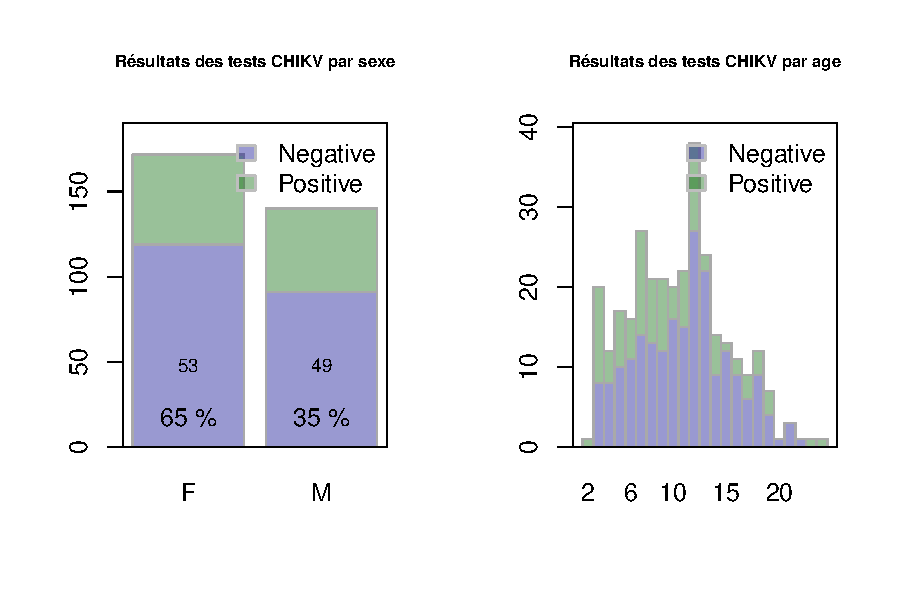
\includegraphics{chik_analyse_pour_madsen-008}
\end{center}
\begin{multicols}{2} 
\setkeys{Gin}{width=0.45\textwidth}




\end{multicols}
\setkeys{Gin}{width=1\textwidth}
%----------------------------------------------------------------------------------------
%  REFERENCE LIST
%----------------------------------------------------------------------------------------
% \newpage
% \bibliographystyle{unsrtnat}
% \bibliography{bibliography}
% 

\end{document}
